\documentclass{article}
\usepackage[pdfcreator={LaTeX}]{hyperref}
\usepackage{graphicx}
\usepackage[utf8]{inputenc} 
\usepackage[ngerman]{babel}

\usepackage[section,toc]{glossaries}\makeglossaries

\newglossaryentry{Regelwerk}{name=Regelwerk,
	plural = Regelwerke,
	description={Regeln eines bestimmten Kartenspiels}
}
\newglossaryentry{Client}{name=Client,
	plural = Clients,
	description={Das Programm, das der Spieler auf seinem Rechner ausführt, um ein Online-Kartespiel zu spielen}
}
\newglossaryentry{Server}{name = Server,
	description={Der zentral ausgeführte Teil der Software, der die Kommunikation und Interaktion mit den Clients verwaltet
		 sowie erstellte Spiele verwaltet und die Einhaltung der Regeln in diesen gewährleistet}
}
\newglossaryentry{Lobby}{name = Lobby,
	description={Ort, an dem Spieler ein Kartenspiel auswählen oder beitreten können}
}
\newglossaryentry{Spielleiter}{name = Spielleiter,
	description={Derjenige, der in der Lobby ein neues Spiel erstellt}
}
\newglossaryentry{Erstellungsfenster}{name = Erstellungsfenster,
	description={Fenster in welchem der Spielleiter das Spiel festlegt}
}
\newglossaryentry{Wartefenster}{name = Wartefenster,
	description={Fenster auf welchem man sich befindet, während man darauf wartet, 
		dass die Mindestteilemerzahl erfüllt ist und das Spiel gestartet wird}
}

\begin{document}
\begin{titlepage}

\begin{center}
\textbf{\textsc{\LARGE Pflichtenheft}}

{\large \today}

\vspace{2cm}
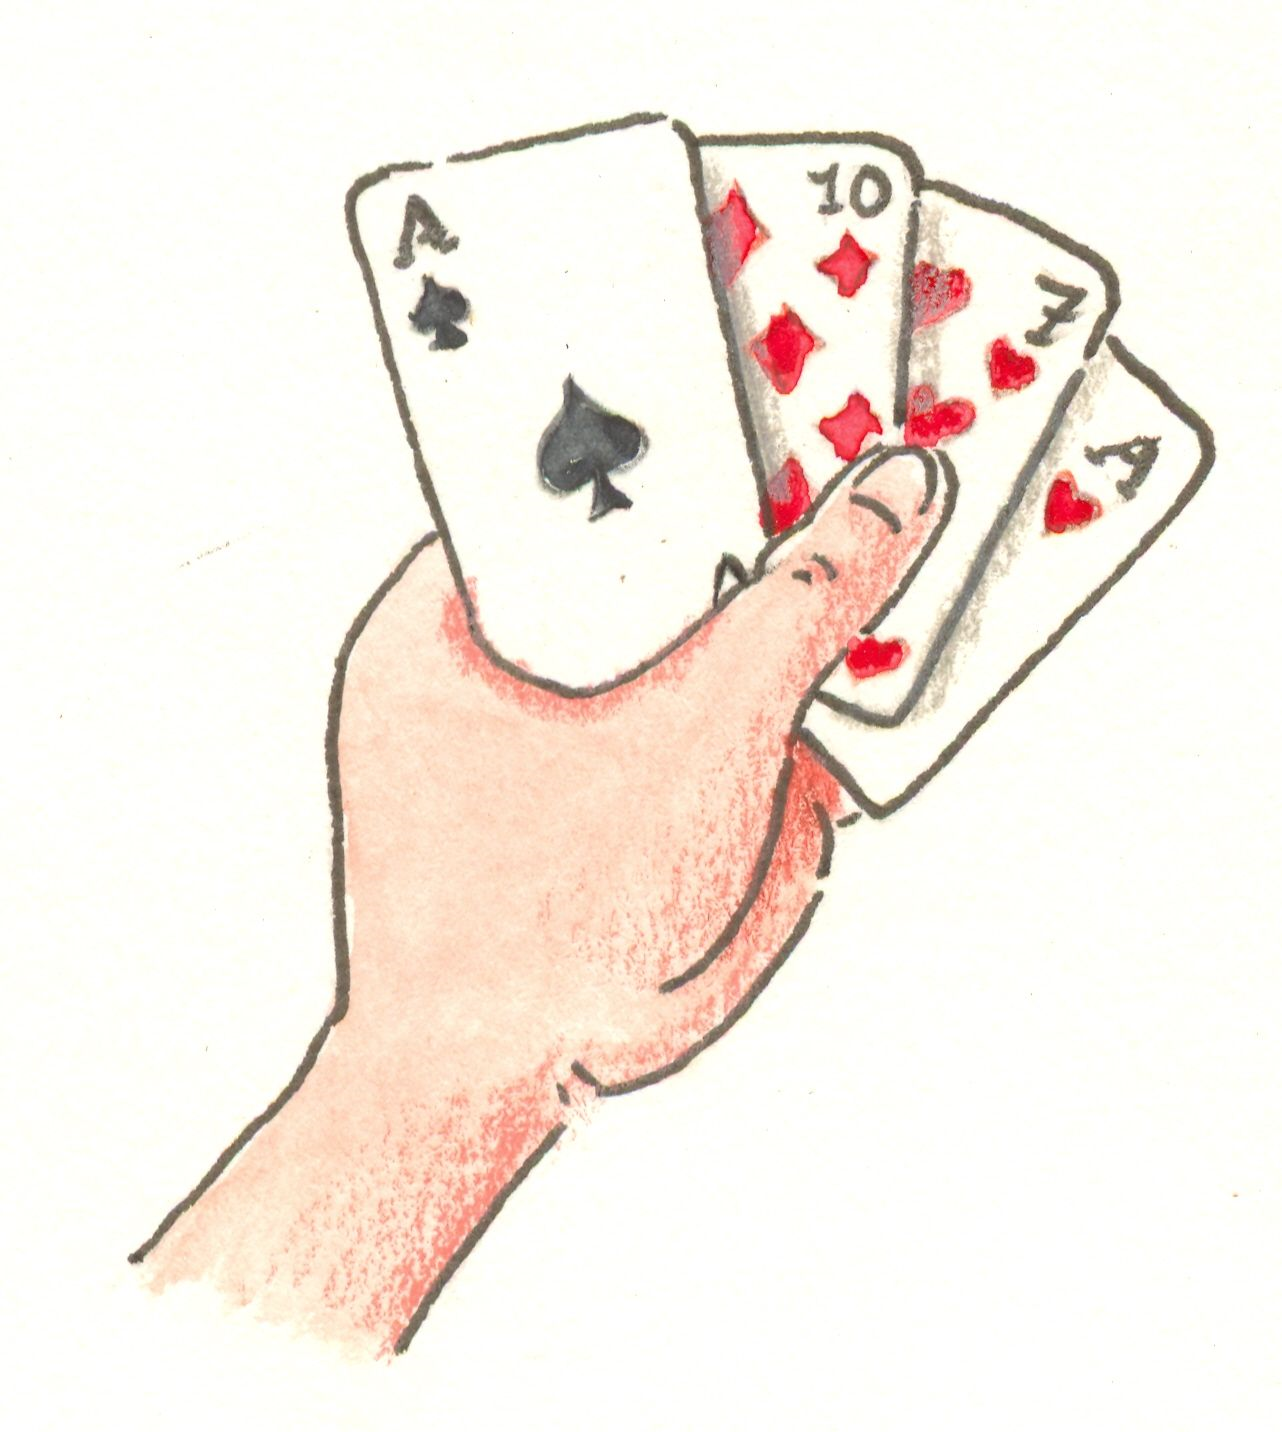
\includegraphics{kartenspiel} 
\ \\
\ \\

\textbf{\textsc{\LARGE NET-WizHearts}}

\vspace{2cm}

\begin{tabular}{|c|c|c|}\hline
   Phase & Verantwortlicher & E-Mail \\ \hline\hline
   Pflichtenheft & Alina  Meixl  &  alina@meixl.de \\ \hline
   Entwurf & Viktoria Witka & witkaviktoria@freenet.de \\ \hline
   Spezifikation & Daniel Riedl & dariedl14@yahoo.de \\ \hline
   Implementation & Andreas Altenbuchner& a.andi007@gmail.com\\ \hline
   Verifikation &Patrick Kubin & kubin@fim.uni-passau.de\\ \hline
   Präsentation & w& w\\ \hline
 \end{tabular}

\end{center}

\end{titlepage}


\tableofcontents
\newpage

\section{Zielbestimmung}
Bei NET-WizHearts handelt es sich um ein Mulitplayer-Online-Kartenspielsystem. Ziel des Produkts ist es eine Basis für mehrere Kartenspiele zu schaffen. So können Spieler mit nur einem einzigen Programm über das lokale Netzwerk oder das Internet miteinander verschiedene \glspl{Regelwerk} spielen. Zusätzlich wird den Spielern die Möglichkeit geboten über Chat zu kommunizieren. Zu Beginn werden bereits Hearts und Wizard als \glspl{Regelwerk} zur Verfügung gestellt.

\subsection{Musskriterien}
Es gibt einen \gls{Server}, der das Spiel verwaltet, und \glspl{Client}, die spielen.
\subsubsection{\gls{Server}}
\begin{itemize}
	\item \glspl{Client} können einen Benutzernamen auswählen und sich anschließend mit dem \gls{Server} verbinden.
		Der Benutzername muss Eindeutig sein, ansonsten wird eine Warnmeldung ausgegeben.
	\item Es gibt eine \gls{Lobby} in der ein Spieler die Möglichkeit hat, Spiele zu erstellen und offenen Spielen beizutreten.
	\item Es gibt einen Chat in der \gls{Lobby}.
	\item Mehrere parallel laufende Spiele auf einem \gls{Server} werden unterstützt.
	\item Regelauswertung mit Überprüfung erlaubter Aktionen, Punktezählung und  Kartenausgabe durch den \gls{Server}.
	\item Die Spiele Hearts und Wizard sind verfügbar.	
	\item Chat mit Mitspielern während eines Spiels ist möglich.
	\item Schutz vor Cheats. Da der \gls{Server} die Kartenverteilung und die Regelauswertung verwaltet, wird es dem 					\glspl{Client} nicht ermöglicht, die Hand eines Mitspielers zu sehen oder die Regeln zu manipulieren.
\end{itemize}

\subsubsection{\gls{Client}}
\begin{itemize}
	\item GUI
	\begin{itemize}
		\item Darstellungsfenster kann mindestens bei der Auflösung von 1024x768 Bildpunkten benutzt werden.
		\item Darstellung des laufenden Spiels. Es wird die eigene Hand offen und die Hände der anderen Spieler verdeckt 					angezeigt. Je nach Spiel gibt es einen allgemeinen Ablagestapel in der Mitte des Spielfeldes oder individuelle 					Ablagestapel vor der Hand des jeweiligen Spielers. Der Zähler für Punktestand, gemachte Stiche, übrige Karten 					etc. befindet sich neben  der Hand des jeweiligen Spielers. Für die Gegenspieler wird zusätzlich der Name über 					der Hand angezeigt.
		\item Eine Karte wird durch einmaliges Anklicken ausgewählt und durch ein zweites Anklicken abgelegt. Es gibt ein extra 					Fenster um die zu verschiebenden Karten bei Hearts bzw. die Stichansage bei Wizard auszuführen.
		\item Die GUI unterstützt den Benutzer sinnvoll  und bietet benutzerfreundliche Eingabeelemente an.
		\item Die Darstellung und das Spiel laufen flüssig.
		\item Die GUI bietet verschiedene Komponenten an, um unterschiedliche \glspl{Regelwerk} zu unterstützen. Dadurch ist es jederzeit möglich neue \glspl{Regelwerk} hinzuzufügen.
		\item Beim Start muss der Spieler einen eindeutigen Benutzernamen auswählen und die IP eines NET-WizHearts \gls{Server}s angeben.
		\item In der \gls{Lobby} werden offene Spiele angezeigt und es gibt die Möglichkeit ein neues Spiel zu erstellen oder 					einem Existierenden beizutreten.
		\item Chat ist in der \gls{Lobby} und während des Spiels möglich
	\end{itemize}
	\item Modell
	\begin{itemize}
		\item Verwaltung der Verbindung mit dem \gls{Server}
		\item Verwaltung des aktuellen Spielzustands (soweit \gls{Client} bekannt)
		\item Vorab-Regelauswertung zur Unterstützung des Nutzers (ungültige Spielaktionen sind nicht durchführbar in der 					GUI)
	\end{itemize}
\end{itemize}

\subsection{Wunschkriterien}
\begin{itemize}
	\item Statistiken, die nach dem Spiel angezeigt werden. Sie zeigen die Plazierung pro Runde.
	\item Mehrere Sprachen werden unterstützt (Deutsch, Englisch, Bayerisch)
	\item Anpassung der GUI durch Spieler ist möglich (Änderung von Hintergrundbild, Kartenrückseite)
	\item Es gibt die Möglichkeit seinem neu erstellten Spiel einen Namen zu geben
	\item Passwortauswahl um Beitritt zu offenen Spielen einzuschränken ist möglich
	\item Nach jedem Spiel kann entschieden werden, ob eine weitere Runde gestartet werden soll
\end{itemize}

\subsection{Abgrenzungskriterien}
\begin{itemize}
	\item Beitreten eines bereits laufenden Spiels nicht möglich
	\item keine Persistenz der Daten über mehrere Sessions, keine Registrierung
	\item keine KI
	\item Spiel wird nicht fortgesetzt, sobald ein Spieler es verlässt
	\item Es werden nur 3-6 Spieler unterstützt
	\item Es gibt keinen Schimpfwortfilter
\end{itemize}

\section{Produkteinsatz}
\subsection{Anwendungsbereich}
Ein Kartenspiel, welches im Freundeskreis oder mit Fremden über das Intenet gespielt werden kann.
\subsection{Zielgruppe}
Personen, die gemeinsam über ein lokales Netzwerk oder das Internet spielen möchten. 
\subsection{Betriebsbedingungen}
Dauerbetrieb der Software.

\section{Produktumgebung}
\subsection{Software}
	\begin{itemize}
		\item \gls{Client}
		\begin{itemize}
			\item Betriebssystem Microsoft Windows, Mac OS X oder Linux-Distribution 
			\item Java 7 Laufzeitumgebung
		\end{itemize}
		\item \gls{Server}
		\begin{itemize}
			\item Betriebssystem Microsoft Windows, Mac OS X oder Linux- Distribution 
			\item Java 7 Laufzeitumgebung
		\end{itemize}
	\end{itemize}

\subsection{Hardware}
\begin{itemize}
		\item \gls{Client}
		\begin{itemize}
			\item Internetfähiger Rechner
		\end{itemize}
		\item \gls{Server}
		\begin{itemize}
			\item Internetfähiger Rechner	
			\item Mindestanforderungen des verwendeten Betriebssystems bezüglich Arbeitsspeicher und Rechenleistung 					      müssen erfüllt sein, können jedoch durch die Anzahl der gehosteten Spieler/Spiele steigen.
		\end{itemize}
	\end{itemize}

\section{Produktfunktionen}
\subsection{Startseite}
\begin{itemize}
	\item /F040/ Auswahl vom gewünschtem \gls{Server} 
	\item /F042/ Auswahl eines eindeutigen Spielernamens
	\item /F045/ Verbinden mit Server (Weiterleitung zur \gls{Lobby})
	\item /F050W/ Auswahl der Sprache
\end{itemize}

\subsection{\gls{Lobby}}
\begin{itemize}
	\item /F060/ Senden einer Nachricht an andere Spieler über den \gls{Server}
	\item /F070/ Ein Spiel auswählen und ihm beitreten. (Bei Passwort geschützten Spiel Weiterleitung zur Passwortabfrage ansonsten Weiterleitung zum \gls{Wartefenster})
	\item /F080/ Erstellen eines neuen Spiels (Weiterleitung zum \gls{Erstellungsfenster})
	\item /F90/ Verlassen der \gls{Lobby} (Programmende)
\end{itemize}

\subsection{\gls{Erstellungsfenster}}
\begin{itemize}
	\item /F120/ Auswahl des \gls{Regelwerk}s
	\item /F122W/ Eingabe eines Namens für das zu erstellende Spiel (Ansonsten wird als Name 'BENUTZERNAME's Spiel' gewählt)
	\item /F124/ Erstellung abbrechen und \gls{Erstellungsfenster} verlassen (Zurückleitung zur \gls{Lobby})
	\item /F126/ Erstellen eines neues Spiels (Weiterleitung zum \gls{Wartefenster})
	\item /F130W/ Möglichkeit ein Passwort für das Spiel zu setzen
\end{itemize}

\subsection{Passwortabfrage}
\begin{itemize}
	\item /F140W/ Eingabe des Passworts.
	\item /F142/ Einem Spiel beitreten (Weiterleitung zum \gls{Wartefenster})
	\item /F145/ Abbrechen (Zurückleitung zur \gls{Lobby})
\end{itemize}

\subsection{\gls{Wartefenster}}
\begin{itemize}
	\item Spieler
	\begin{itemize}
		\item /F160/ Chat mit anderen Spielern im selben Spiel
		\item /F170/ Verlassen des Spiels (Zurückleitung zur \gls{Lobby})
	\end{itemize}
	\item \gls{Spielleiter}
	
	Besitzt alle Funktionen des Spielers
	\begin{itemize}
		\item /F180/ Spieler entfernen
		\item /F190/ Auflösung des Spiels durch Verlassen des \gls{Wartefenster}s (Zurückleitung zur \gls{Lobby})
		\item /F200/ Starten des Spiels (Voraussetzung: Mindestanzahl der Spieler erreicht)
	\end{itemize}
\end{itemize}

\subsection{Spiel}
\begin{itemize}
	\item Alle Spiele
	\begin{itemize}
		\item /F210/ Verlassen des Spiels (Zurückleiten aller Spieler zur \gls{Lobby})
		\item /F220/ Nachricht senden an andere Spieler
		\item /F225/ Karte auswählen (Voraussetzung: Spieler am Zug und Karte darf gespielt werden)
		\item /F230/ Karte spielen (Voraussetzung: Karte ausgewählt)
		\item /F240/ Veränderungen der GUI vornehmen
	\end{itemize}
	\item Hearts
	\begin{itemize}
		\item /F260/ Auswahl der Karten, die weitergeschoben werden sollen.
	\end{itemize}
	\item Wizard
	\begin{itemize}
		\item /F360/ Auswahl der Trumpffarbe zu Beginn einer Runde (Voraussetzung: Aufdecken des Zauberers)
		\item /F370/ Eingabe der gewünschten Stiche zu Beginn jeder Runde
	\end{itemize}
\end{itemize}

\section{Produktdaten}
\subsection{\gls{Regelwerk}e}
\subsubsection{/D010/ Hearts}	
\begin{itemize}
	\item Kartenstapel
	\begin{itemize}
		\item Kartenanzahl: 52
		\item Karten:
		\begin{itemize}
			\item Farbe: Kreuz, Pik, Herz, Karo
			\item Wertigkeit: 2-10, Bube, Dame, König, Ass
			\item Punkte: Herz = 1 Punkt, Pik Dame = 13 Punkte, Andere = 0 Punkte
		\end{itemize}	
		\item Kartenverteilung pro Runde: 13 Karten				
	\end{itemize}
	\item Erlaubte Spieleranzahl: 4 Spieler		
	\item Spieler /D010/
	\begin{itemize}
		\item Karten
		\item Punktestand (Bei 100 Punkte Spielende)
		\item Kreuz 2 Regel (Muss bei Besitz gespielt werden, beginnt das Spiel)
		\item Status (Am Zug, Wartend)
	\end{itemize}
	\item Runden
	\item Tauschreihenfolge	
	\item Ablagestapel:
	\begin{itemize}
		\item Zugreihenfolge
		\item Spielbare Karten
		\item Stichvergabe an Spieler
		\item Anzeigedauer der Karten
	\end{itemize}
	\item Platzierung der Spieler nach Punkten
\end{itemize}
	
\subsubsection{/D020/ Wizard}
\begin{itemize}
	\item Kartenstapel
	\begin{itemize}
		\item Kartenanzahl: 60
		\item Karten
		\begin{itemize}
			\item Reguläre Karten
			\begin{itemize}
				\item Farbe: blau, rot, grün, gelb
				\item Wertigkeit: 1-13	
			\end{itemize}
			\item Sonderkarten
			\begin{itemize}
				\item Zauberer: 4 Karten
				\item Narr: 4 Karten
			\end{itemize}			
		\end{itemize}	
		\item Kartenverteilung pro Runde: 1 plus eine für jede weitere Runde
	\end{itemize}
	\item Spieleranzahl: 3-6
	\item Spieler /D010/
	\begin{itemize}
		\item Karten
		\item Stiche
		\item Stichvorhersage
		\item Punkte
		\item Status (Am Zug, Wartend)
	\end{itemize}
	\item Runden
	\begin{itemize}
		\item Anzahl: 20, 15, 12, 10 (Abhängig von Spieleranzahl)
		\item Trumpffarbe
		\item Anfangsspieler
		\item Spielende bei letzter Runde
	\end{itemize}
	\item Ablagestapel
	\begin{itemize}
		\item Zugreihenfolge
		\item Spielbare Karten
		\item Stichvergabe an Spieler
		\item Anzeigedauer der Karten
	\end{itemize}
	\item Platzierung der Spieler nach Punkten
\end{itemize}

\subsection{Andere Daten}
\subsubsection{/D030/ Spieler}
\begin{itemize}
	\item Spielername (eindeutig)
	\item \gls{Server}
	\item Sprache
	\item Status (\gls{Lobby}, Spiel)
\end{itemize}	

\subsubsection{/D040/ Spiel}
\begin{itemize}
	\item Spielname
	\item Spieler /D030/
	\begin{itemize}
		\item \gls{Spielleiter}
		\item Andere Spieler
	\end{itemize}
	\item Spieleranzahl
	\item \gls{Regelwerk} /D010/ oder /D020/
	\item Chatinhalt
	\item Status(Erstellung, Laufend, Ende)
	\item Passwort(optional)
\end{itemize}

\subsubsection{/D050/ \gls{Lobby}}
\begin{itemize}
	\item Spieler /D010/ (Status = \gls{Lobby})
	\item Spiele /D040/ (Status = Erstellung)
	\item Chatinhalt
\end{itemize}

\section{Produktleistungen}
\subsection{\gls{Lobby}}
\begin{itemize}
	\item /L100/ Anzeige der Namen eingeloggter Spieler, die noch keinem Spiel beigetreten sind
	\item /L110/ Anzeige von erstellten Spielen (Spielname, Spielerzahl, Spieltyp)	
	\item /L115/ Anzeige des Chatdialoges		
\end{itemize}

\subsection{\gls{Erstellungsfenster}}
\begin{itemize}
	\item /L120/ Anzeige eines Spiellogos
	\item /L122/ Anzeige einer kurzen Spielbeschreibung (bei Mouseover über das Logo)
\end{itemize}

\subsection{\gls{Wartefenster}}
\begin{itemize}
	\item /L150/ Anzeigen des Spieltyps
	\item /L155/ Anzeigen der Mitspieler
	\item /L158/ Anzeige des Chatdialoges
	\item /L170/ Spiel wird aufgelöst wenn der \gls{Spielleiter} selbst das Spiel verlässt
\end{itemize}

\subsection{Spiel}
\begin{itemize}
	\item /L190/ Anzeige der eigenen Karten
	\item /L192/ Anzeige der verdeckten Karten der Mitspieler
	\item /L194/ Anzeige des Ablagestapels
	\item /L195/ Anzeige des Aufnahmestapels
	\item /L198/ Anzeige der Anzahl der restlichen Karten für jeden Spieler bzw. Anzahl der vorhergesagten sowie bereits erspielten Stiche
	\item /L200/ Anzeige des Punktestandes
	\item /L250W/ Anzeige einer Auswertung nach Beendigung einer Runde oder eines Spiels
	\item /L260/ Anzeige des Chatdialoges
	\item /L275W/ Nach Spielende wird per Votum entschieden, ob ein neues Spiel begonnen wird.
	\item /L280/ Einhaltung der Spielregeln gewährleisten
\end{itemize}

\subsection{\gls{Server}}
\begin{itemize}
\item /L300/ Verwaltung mehrerer parallel laufender Spiele
\item /L330/ Schutz vor Cheats: Regelauswertung durch Server, Handkarten aller Spieler nur dem \gls{Server} bekannt 
		(\gls{Client} kennt nur eigene Handkarten)
\end{itemize}
	
\subsection{Allgemein}
\begin{itemize}
	\item /L270/ Nutzen des Chatdialoges zur Benachrichtigung der Spieler über Ereignisse
	\item /L290/ Fehlermeldungen bei ungültigen Nutzeraktionen ausgeben
	\item /L350W/ Mehrsprachigkeit unterstützen
	\item /L380/ Bei Programmende Benutzername löschen
\end{itemize}
	

\section{Benutzeroberfläche}
\begin{itemize}
	\item Startseite:  Auf dieser Seite kann sich der Spieler einen Benutzernamen aussuchen und sich mit dem \gls{Server} verbinden. Außerdem legt er die Sprache für das gesamte Programm fest.\\ 				\ \\
		\makebox[\textwidth]{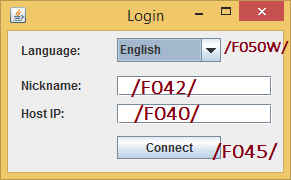
\includegraphics{GUI_images/Login}}
		\ \\
	\item \gls{Lobby}: In der \gls{Lobby} können Spieler mit den unteren Buttons ein neues Spiel erstellen,  einem offenem Spiel 					beitreten oder die \gls{Lobby} verlassen. In der linken Spalte sind die Spieler zu sehen, die sich gerade in der 					\gls{Lobby} befinden. In der rechten Spalte sieht 					man die offenen Spiele, mit momentaner Spielerzahl und und Spieltyp. Im unteren Teil der \gls{Lobby} ist der Chat.\\
		\ \\
		\makebox[\textwidth]{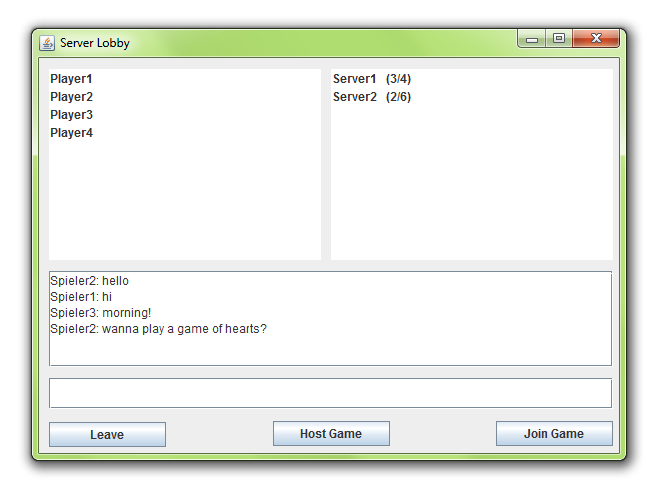
\includegraphics[scale=0.7]{GUI_images/ServerLobby}}
		\newpage
	\item \gls{Erstellungsfenster}: Im \gls{Erstellungsfenster} kann der \gls{Spielleiter} ein neues Spiel erstellen. Dabei muss er ein 			\gls{Regelwerk} aussuchen und kann wahlweise dem Spiel einen Namen geben und das Passwort setzen. Fährt 					der \gls{Spielleiter} mit der Maus über das Bild, wird ein kurzer beschreibender Text zu dem jeweiligen Spiel 					gezeigt.\\
		\ \\
		\makebox[\textwidth]{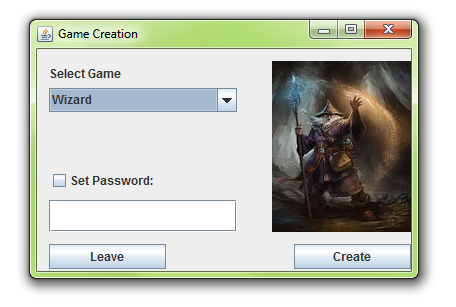
\includegraphics[scale=0.8]{GUI_images/CreateGame}}
		\ \\
	\item \gls{Wartefenster}: Im \gls{Wartefenster} befinden sich die Personen, die einem offenem Spiel beigetreten sind. Sobald 					die Mindestspielerzahl erreicht ist kann ein neues Spiel gestartet werden. Für das \gls{Wartefenster} ist ein eigener 					Chat verfügbar. Man kann das \gls{Wartefenster} auch mit einem der unteren Buttons verlassen. \\
		\ \\
		\makebox[\textwidth]{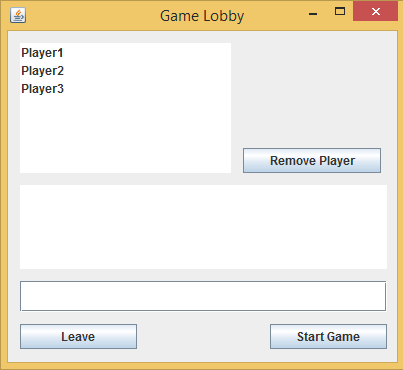
\includegraphics[scale=0.7]{GUI_images/GameLobby}}
		\ \\
	\item Passwortabfrage: Bevor die Spieler einem passwortgeschützem Spiel beitreten können, müssen sie das Passwort, das der 						\gls{Spielleiter} festgelegt hat, in das Textfeld eingeben.\\
		\ \\
		\makebox[\textwidth]{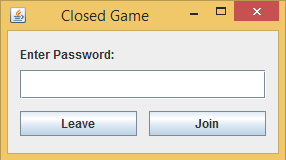
\includegraphics{GUI_images/PasswordRequest}}
		\ \\
	\item Spiel: Im Spielfeld wird die eigene Hand offen und die der anderen Spieler verdeckt angezeigt. Je nach Spiel gibt es 					einen allgemeinen Ablagestapel in der Mitte des Spielfeldes oder individuelle Ablagestapel vor der Hand des 					jeweiligen Spielers. Die Zähler für Punktestand und gemachte Stiche oder übrige Karten etc. befindet sich neben  der 					Hand des jeweiligen Spielers. Für die Gegenspieler wird zusätzlich der Name über der Hand angezeigt.\\
			Im unteren Bereich gibt es ein Chatfenster für die Mitspieler. Oben links soll man im Dropdown-Menü unter dem Punkt 'Einstellungen' die Hintergrundbilder anpassen können.\\
		\ \\
		\makebox[\textwidth]{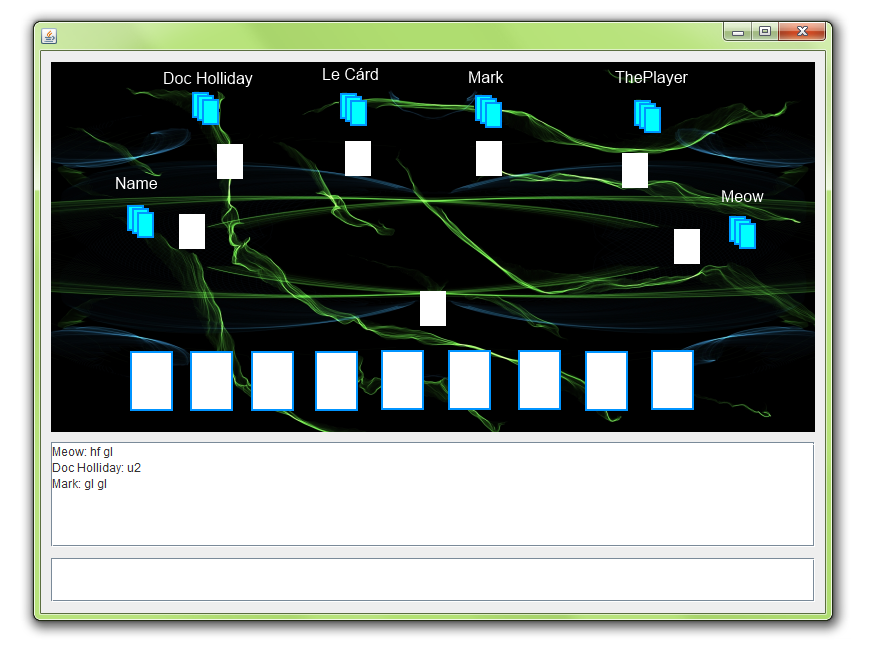
\includegraphics[scale=0.6]{GUI_images/GameClient}}
\end{itemize}

\section{Testszenarien}
\begin{itemize}
	\item Startseite (keine Vorraussetzungen): \\
	\begin{itemize}
	
		\item /T020/ \textit{Verbindungsaufbau mit \gls{Server}:} Mr. Blue gibt den Nickname 'MrBlue' und die Adresse des \gls{Server}s ein (/F040/). Er verbindet sich mit dem \gls{Server} und gelangt die \gls{Lobby} (/F045/). 
		
		\item /T025/ \textit{Falsche Eingabe (Name):} Mr. Blue gibt keinen Namen ein, es kommt zu einer Fehlermeldung (/L290/ 'Kein Name angegeben').
		
		\item /T027/ \textit{Falsche Eingabe (Name):} Nachdem Mr. Blue schon auf dem \gls{Server} eingeloggt ist, versucht nun Mr. Bleau sich mit dem Nickname 'MrBlue' einzuloggen. Es wird eine Fehlermeldung angezeigt (/L290/ 'Name wird bereits verwendet').
		
		\item /T029/ \textit{Falsche Eingabe (IP):} Mr. Blue vertippt sich beim Eingeben der \gls{Server}radresse. Beim Loginversuch wird ein Fehler ausgegeben (/L290/ '\gls{Server} konnte nicht gefunden werden').
		
		\item /T030/ \textit{Auswahl der Sprache:} Mr. Blue wählt im Dropdown-Menü die Sprache 'English' aus (/F050W/), das Login-Fenster wird neu erstellt und es und alle folgenden Fenster sind nun in englischer Sprache.
	\end{itemize}
	
		\item /T035/ \textit{Beenden und wieder Einloggen:} Mr. Blue ist mit dem Namen 'MrBlue' eingeloggt. Er beendet das Spiel und der Nickname wird wieder freigegeben (/L380/). Er startet das Spiel noch einmal und loggt sich wieder mit 'MrBlue' ein (/F045/)

	\item \gls{Lobby} (Vorraussetzungen: /T020/: \\ \\
	\begin{itemize}
	
		\item /T040/ \textit{Spielerliste:} Der eigene Benutzername 'MrBlue' und die Benutzernamen aller anderen verbundenen \gls{Client}s werden sofort in der Spielerliste angezeigt (/L100/).
		
		\item /T050/ \textit{\gls{Server}liste:} Alle von Nutzern erstellten Spiele werden in der Spielliste angezeigt (/L110/).
	
		\item /T060/ \textit{Chatnachricht senden:} Mr. Blue gibt die Nachricht 'Hallo Kartenwelt!' in das untere Textfeld ein und drückt die Entertaste (/F060/). Im oberen Textfeld wird die aktuellste Nachricht und alle bisher gesendeten Nachrichten angezeigt (/L115/). Mr. Pink ist auch in der \gls{Lobby}, sieht die Nachricht von Mr. Blue (/L115/) und sendet die Nachricht 'Hallo MrBlue' (/F060/). Diese erscheint ebenfalls im Chat aller Spieler(/L115/).
		
		\item /T080/ \textit{Spiel erstellen:} Mr. White erstellt ein Spiel und gelangt ins \gls{Erstellungsfenster} (/F080/).
		
		\item /T085/ \textit{Mehrere Spiele erstellen (Vorrausetzung: /T080/, /T110/):} Mr Pink erstellt ein weiteres Spiel und gelangt ins \gls{Erstellungsfenster} (/F080/). Für alle eingeloggten Spieler sind nun beide Spiele sichtbar.
		
		\item /T090/ \textit{Spiel beitreten:} Mr. Blue tritt dem bereits korrekt geöffneten und noch nicht vollen Spiel von Mr. White bei und gelangt ins \gls{Wartefenster} (/F070/).
		
		\item /T092/ \textit{Fehler bei Spiel beitreten:} Mr. Brown hat kein Spiel aus der Liste ausgewählt. Er drückt den 'Join'-Knopf und es wird eine Fehlermeldung angezeigt (/L290/ 'Kein Spiel ausgewählt').
		
		\item /T095/ \textit{Passwortabfrage:} Das Spiel von Mr. White ist passwortgeschützt. Mr. Blue gibt 'youshouldtip' in das zugehörige Textfeld ein (/F140/) und drückt den 'Join'-Knopf, wodurch er zum \gls{Wartefenster} weitergeleitet wird (/F142/). 
		
		
		\item /T097/ \textit{Passwortabfrage(Abbruch):} Das Spiel von Mr. White ist passwortgeschützt. Mr. Blue kennt das Passwort nicht. Er gibt 'damn' in das Textfeld ein und drückt den 'Join'-Knopf. Eine Fehlermeldung erscheint (/L290/ 'Falsches Passwort') und er bleibt in der Passwortabfrage. Er den 'Cancel'-Knopf und gelangt zurück in die \gls{Lobby} (/F145/).
			  
	\end{itemize}
	\ \\
	\item Erstellungsfenster (Vorraussetzung: /T080/): 
	
	\begin{itemize}
	
		\item /T100/ \textit{\gls{Regelwerk} auswählen:} Mr. White wählt 'Wizard' als \gls{Regelwerk} aus (/F120/) und schaut sich dessen Logo an (/L120/), sowie eine kurze Beschreibung des Spiels, die erscheint, wenn er mit der Maus über das Logo fährt (/L122/).
		
		\item /T105/ \textit{\gls{Regelwerk} auswählen:} Mr. White wählt 'Hearts' als \gls{Regelwerk} aus (/F120/) und schaut sich dessen Logo an (/L120/), sowie eine kurze Beschreibung des Spiels, die erscheint, wenn er mit der Maus über das Logo fährt (/L122/).
		
		\item /T110/ \textit{Spiel erstellen:} Mr. White gibt 'NewHeist' als Spielname ein (/F122/). Er setzt einen Haken bei 'Passwort' und gibt 'youshouldtip' als Passwort ein (/F130W/). Er drückt auf den 'Create'-Knopf, erstellt somit ein Spiel und wird zum \gls{Wartefenster} weitergeleitet (/F126/).
		
		\item /T115/ \textit{Spiel erstellen:} Mr. White gibt keinen Spielnamen an. Bei drücken des 'Create'-Knopfes wird ein Spiel mit dem Namen 'MrWhite`s Spiel' erstellt.
		
		\item /T117/ \textit{Fehler bei Spiel erstellen:} Mr. White gibt 'NewHeist' als Spielname ein (/F122/). Er setzt einen Haken bei 'Passwort', aber vergisst ein Passwort einzugeben. Bei drücken des 'Create'-Knopfes wird eine Fehlermeldung angezeigt (/L290/ 'Kein Passwort gewählt').
		
		\item /T120/ \textit{Erstellung abbrechen:} Mr. White erfährt, dass Mr. Pink schon in einem anderen Spiel ist und entschließt sich die Erstellung abzubrechen. Er drückt den 'Cancel'-Knopf und gelangt zurück in die \gls{Lobby} (/F124/).
	
	\end{itemize}
	
	\item \gls{Wartefenster} (Vorraussetzung: /T110/, /T090/)
	
	\begin{itemize}
		
		\item /T130/ \textit{Chat:} Mr. Pink und Mr. White befinden sich im \gls{Wartefenster} des Spiels. Mr. Pink schreibt die Chatnachricht 'Hello Mr. White' und sie wird bei beidem im Chat angezeigt (/F160/).
		
		\item /T170/ \textit{Verlassen:} Mr. Brown ist gerade dem Spiel beigetreten und verlässt es sofort wieder. Im Chat wird 'MrBrown ist dem Spiel beigetreten' angezeigt (/L270/). Er gelangt zurück in die \gls{Lobby} (/T170/). Mr. White und Mr. Pink sehen den Namen 'MrBrown' kurz in der Spielerliste, bevor er wieder verschwindet.
		
		\item /T180/ \textit{Spieler entfernen:} Mr. Blue tritt dem Spiel bei. Mr. Pink hat das Spiel erstellt. Er ist somit \gls{Spielleiter} und entschließt sich dazu Mr. Blue aus dem Spiel zu werfen (/F180/). Nach Drücken des 'Remove Player'-Knopfes gelangt Mr. Blue wieder in die \gls{Lobby}. Mr. Blue erhält die Nachricht 'Sie wurden vom Spiel entfernt'. Im Chat wird angezeigt 'MrPink hat MrBlue vom Spiel entfernt'(/L270/).
		
		\item /T182/ \textit{Fehler bei Spieler enntfernen:} Mr. Pink ist \gls{Spielleiter}. Er drückt den 'Remove Player'-Knopf, hat aber keinen Spieler ausgewählt. Es wird eine Fehlermeldung angezeigt (/L290/ 'Kein Spieler ausgewählt').
		
		\item /T185/ \textit{Fehler bei Starten des Spiels:} Mr. White ist allein im \gls{Wartefenster}. Er drückt auf den 'Start'-Knopf und es wird eine Fehlermeldung angezeigt (/L290/ 'Nicht genügend Spieler').
		
		\item /T190/ \textit{Spiel starten:} Mr. Brown und Mr. Orange treten dem Spiel bei. Es sind nun genug Spieler vorhanden, deshalb entschließt sich Mr. Pink dazu, das Spiel zu starten (/F200/). Alle Spieler gelangen ins Spielfenster, das \gls{Wartefenster} wird geschlossen.
		
		\item /T200/ \textit{Spiel auflösen:} Es dauert Mr. Pink zu lange, bis genug Spieler zusammenkommen, also verlässt er das \gls{Wartefenster}. Da er der \gls{Spielleiter} war, wird das Spiel aufgelöst und alle Spieler gelangen zurück zur \gls{Lobby} (/F190/).
		 
	\end{itemize}

	\item Spielfenster Allgemein(Voraussetzung: /T190/)
	
	\begin{itemize}
	
		\item /T210/ \textit{Spielbeginn (Voraussetzung: /T100/):} Mr. Pink, Mr. White, Mr. Brown und Mr. Orange befinden sich im Spielfenster. Der \gls{Server} teilt die Karten aus. Jeder sieht seine, ihm vom \gls{Server} ausgeteilten Karten (/L190/) und die verdeckten Karten seiner Mitspieler (/L192/).  

		\item /T220/ \textit{Zug: (Voraussetzung: /T210/)} Mr. Pink ist nicht am Zug, jedoch versucht er dennoch eine Karte zu spielen, was mit einem entsprechendem Dialog  unterbunden wird (/L290/).
		
		\item /T240/ \textit{Hintergrund ändern:} Mr. Pink klickt im Dropdown-Menü auf 'Einstellungen'. Ein Dialog mit eine Pfadabfrage öffnet sich. Mr. Pink gibt die Datei './neuerHintergrund.png' im Pfad an. Der Hintergrund des Spielfelds zeigt diese Bild an.
		
		\item /T270/ \textit{Spielende:} Mr. Orange spielt die letzte Karte des Spiels. Das Spiel ist zu Ende und der \gls{Server} bestimmt den Gewinner. Mr. Orange bekommt eine Zusammenfassung angezeigt, die ihn als Sieger erklärt und seine Punkte anzeigt(/L250/). Alle anderen Spieler erhalten ebenfalls eine Zusammenstellung ihrer Leistung (/L250/).
		
		\item /T280/ \textit{Spielabbruch: (Voraussetzung /T190/)} Es läuft für Mr. Pink nicht sonderlich gut und er entschließt sich, es sein zu lassen, weshalb er das Spiel durch einen Klick auf 'schließen' beendet und sich anschließend in der \gls{Lobby} wiederfindet (/F210/). Mr. White, Mr. Brown und Mr. Orange werden über das Verlassen des Spielers 'Mr. Pink' durch eine Fehlermeldung informiert (/L290/) und werden ebenfalls in die \gls{Lobby} zurückgeworfen.
	
		\item /T300/ \textit{Chat:} Mr. Pink, Mr. White, Mr. Brown und Mr. Orange befinden sich im Spielfenster. Mr. Orange schreibt die Chatnachricht 'Hallo zusammen!' (/F220/) und sie wird bei allen im Chat angezeigt (/L260/).
	
		\item /T310/ \textit{Chat:} Mr. Pink, Mr. White, Mr. Brown und Mr. Orange befinden sich im Spielfenster. Mr. Orange versucht eine leere Nachricht im Chatfenster abzusetzen, die Nachricht wird nicht gesendet und erscheint auch nicht in seinem Chat.
		
		\item /T320/ \textit{Neue Runde:} Das Spiel wurde fertig gespielt. Jeder Mitspieler erhält eine Abfrage ('Nochmal spielen?') (/L275W/). Jeder Spieler stimmt mit 'Ja'. Es wird ein neues Spiel gestartet (/F200/).
			
	\end{itemize}
	
	\item Spielfenster Wizard
	
	\begin{itemize}
	
		\item /T228/ \textit{Rundenbeginn: (Vorraussetzung: /T210/)} Der \gls{Server} dreht die oberste Karte auf dem Aufnahmestapel (/L195/) automatisch um und sagt dadurch die Trumpffarbe (ausgenommen einen Zauberer) an. Im Chat erscheint eine Spielnachricht des \gls{Server}s (/L270/).

		\item /T230/ \textit{Stiche ansagen: (Voraussetzung: /T228/)} Nach längerem Spiel wird einer der 4 Zauberer vom \gls{Server} beim Kartengeben aufgedeckt und da Mr. Pink an der Reihe ist, erscheint ein Auswahlfenster. Mr. Pink wählt die Trumpffarbe. (/F360/) Über den Spielchat erhalten alle Spieler Auskunft über den Vorgang (/L270/) und sehen die angesagte Farbe.
	
		\item /T240/ \textit{Stiche ansagen: (Voraussetzung: /T228/ oder /T230/)} Nachdem eine Trumpffarbe angesagt wurde erscheint ein Fenster, indem jeder Spieler die Anzahl seiner Stiche tippen kann. Mr. Brown glaubt 4 Stiche machen zu können und gibt die Zahl ein (/F370/). Auch die anderen Spieler geben ihre Tipps ab und sehen die prognostizierten Stiche der anderen.(/L196/).
		
		\item /T245/ \textit{Stiche ansagen:(Voraussetzung: /T228/ oder /T230/)} Nachdem eine Trumpffarbe angesagt wurde erscheint ein Fenster, indem jeder Spieler die Anzahl seiner Stiche tippen kann. Mr. Orange gibt 'zehn' in das Feld ein. Es wird eine Fehlermeldung angezeigt (/L290/ 'Bitte geben sie eine Zahl ein').

		\item /T250/ \textit{Rundenbeginn: (Voraussetzung: /T210/)} Der Server gibt die Karten und dreht die oberste Karte auf dem Aufnahmestapel (/L195/) automatisch um und sagt dadurch die Trumpffarbe (ausgenommen einen Zauberer) an. Im Chat erscheint eine Spielnachricht des \gls{Server}s (/L270/).
		
				\item /T260/ \textit{Rundenende:} Mr. Pink spielt die letzte Karte der Runde. Es erscheint eine kurze Zusammenfassung, wie viele Stiche er gemacht hat, wie viele er getippt hat und erhält seinen aktuellen Punkestand sowie den der anderen Mitspieler in einem separatem Fenster angezeigt (/L250/).
					
	\end{itemize}
	
	\item Spielfenster Hearts
	
	\begin{itemize}
	
		\item /T290/ \textit{Spielbeginn Hearts: (Voraussetzung /T105/)} Mr. Pink, Mr. White, Mr. Orange und Mr. Brown befinden sich im Spielfenster. Das Spiel beginnt und ein Fenster erscheint bei allen Spielern indem 3 Karten ausgewählt werden müssen. Mr. White wählt 3 Karten aus und bestätigt seine Auswahl (/F260/). Nachdem Mr. Orange ebenfalls 3 Karten zur Weitergabe ausgewählt hat erhält diese Mr. White. Mr. Pink erhält die 3 Karten von Mr. White und  Mr. Orange erhält die Karten von Mr. Pink.

		\item /T295/ \textit{Spielbeginn Hearts: (Voraussetzung /T105/)} Mr. Pink, Mr. White, Mr. Orange und Mr. Brown befinden sich im Spielfenster. Das Spiel beginnt und ein Fenster erscheint bei allen Spielern, in dem 3 Karten ausgewählt werden müssen. Mr. White nur 2 Karten aus und bestätigt seine Auswahl (/F260/). Es erscheint ein Dialog der ihn auffordert 3 Karten auszuwählen(/L290/).

		\item /T330/ \textit{Zug: (Vorausetzung /T210/)} Mr. Pink versucht eine ungültige Karte zuzugeben. Das Spiel erkennt den Regelverstoß und zeigt dies über einen Dialog an (/L290/).
	\end{itemize}
\end{itemize}

\section{Entwicklungsumgebung}
\subsection{Software}
\begin{itemize}
	\item LaTeX
	\item Eclipse
	\item IBM Rational Software Architect
	\item Git
\end{itemize}

\subsection{Hardware}
\begin{itemize}
	\item Rechner im CIP Pool	
	\item Private Rechner
\end{itemize}

\section{Qualitätsbestimmungen}

\begin{itemize}
\item Benutzerfreundlichkeit:

Das Interface sollte intuitiv bedienbar sein und ohne weitere Hilfe für den Benutzer nachvollziehbar sein, daher ist Benutzerfreundlichkeit ein sehr wichtiges Kriterium. Sie wird garantiert durch eine Übersichtliche Gestaltung der GUI und präzise Fehlermeldungen bei falscher Interaktion. 

\item Performanz

Da die Anwendung keine allzu großen Berechnungen durchführen sollte, ist die Performanz des Programms zwar wichtig aber hat nicht die höchste Priorität.

\item Erweiterbarkeit/Evolution

Im den Muss-Kriterien wird explizit darauf hingewiesen, dass es ohne großen Aufwand möglich sein sollte weitere \glspl{Regelwerk} hinzuzufügen. Dies wird gewährleistet, indem neue GUI-Elemente (z.B. Abfragen, Anzeigen), die vom \gls{Regelwerk} benötigt werden, modular hinzugefügt werden können.

\item Korrektheit

Um die Fairness in einem Spiel aufrecht zu erhalten, sollten keine Fehler auftauchen, die gegen die Regeln des Spiels verstoßen. Das Spiel muss seine eigenen Regeln auch einhalten!

\item Sicherheit

Da dies ein eher kleines Programm ist deren Zielgruppe auch nicht groß ist, werden auch keine größeren Sicherheitsmaßnahmen vorgenommen. Korrekte Einhaltung der Regeln wird vom \gls{Server} gewährleistet.

\item Stabilität

Ein instabiles Programm, in dem es vielfach zu Spielabstürzen oder anderen lästigen Fehlern kommt, wäre für den Benutzer sehr ärgerlich und würde den Spielspass sehr eindämpfen. Es ist daher wichtig, dass das Programm robust läuft.

\item Übertragbarkeit

Die Übertragbarkeit der Anwendung ist durch die Verwendung von Java gegeben.

\end{itemize}
\newpage
\printglossaries
\end{document}
